\documentclass[12pt]{article}

\usepackage{sbc-template}

\usepackage{graphicx,url}
\usepackage[utf8]{inputenc}
\usepackage[brazilian]{babel}
\usepackage{float}
\usepackage{verbatim}

\sloppy

\title{Avaliação Experimental da Capacidade de LLMs na Resolução de Problemas na Modalidade Programação da Olimpíada Brasileira de Informática}

\author{Victor Hugo S. Ângelo\inst{1}, Ricardo Vinicius A. Fernandes\inst{1}, Matheus Ryan S. Nascimento\inst{1}, Lucas Heron S. Anchieta\inst{1}, Evandro de B. Costa\inst{1}}

\address{Instituto de Computação -- Universidade Federal de Alagoas (UFAL)\\
  Av. Lourival Melo Mota, S/N, Maceió - AL
  \email{\{vhsa,rvaf,mrysn,lhsa, evandro\}@ic.ufal.br}
}

\begin{document}
\maketitle

\begin{abstract}
This article evaluates the capability of Large Language Models (LLMs) in solving complex algorithmic challenges from the Brazilian Olympiad in Informatics (OBI). For this research, an automated experimental environment was created, comprising a code-generating agent and a judge for test case validation. The results indicate that the models easily master basic-level questions but present severe limitations in advanced topics. Furthermore, the use of examples in the prompt is essential to guide the outputs of the LLMs. Finally, the research maps the actual capabilities and cognitive limits of these tools, providing a solid foundation for the future integration of LLMs to support competitive programming education.
\end{abstract}
     
\begin{resumo}
Este artigo avalia a capacidade de Modelos de Linguagem (LLMs), na resolução de desafios algorítmicos complexos da Olimpíada Brasileira de Informática (OBI). Para a pesquisa, criou-se um ambiente experimental automatizado composto por um agente gerador de código e um juiz para validação dos casos de teste. Os resultados indicam que os modelos dominam facilmente as questões de nível básico, mas apresentam limitações severas em tópicos avançados. Além disso, o uso de exemplos no prompt é essencial para guiar as saídas das LLMs. Por fim, a pesquisa mapeia as reais capacidades e os limites cognitivos dessas ferramentas, fornecendo uma base sólida para a futura integração de LLMs no suporte ao ensino de programação competitiva.
\end{resumo}

\section{Introdução}

A resolução de problemas de programação é uma atividade cognitiva complexa que exige não apenas o domínio da sintaxe de uma linguagem, mas, sobretudo, competências avançadas de raciocínio lógico, abstração e conhecimento algorítmico. No cenário educacional brasileiro em computação, a Olimpíada Brasileira de Informática (OBI) destaca-se como um dos instrumentos de fomento a essas competências, desafiando estudantes a resolverem problemas de programação de alta complexidade sob restrições rigorosas de tempo e memória.

Paralelamente, o surgimento e a rápida evolução dos Modelos de Linguagem de Grande Escala (LLMs) têm influenciado a área de engenharia de software, demonstrando capacidades impressionantes na geração de código e na tradução de requisitos de linguagem natural para linguagens de programação. Entretanto, a aplicação dessas ferramentas em contextos de programação competitiva ainda apresenta lacunas de desempenho significativas. Nesses cenários, os enunciados frequentemente exigem interpretação semântica profunda e a construção de cadeias complexas de raciocínio, demandando o uso de técnicas avançadas, como programação dinâmica ou teoria dos grafos, ainda apresenta lacunas de desempenho significativas. Embora estudos nacionais e internacionais investiguem a capacidade de LLMs em resolução de problemas em variados contextos e domínios \cite{chen2021evaluating, mendonca2024evaluating, viegas2025assessing, huang2024competition, zheng2025livecodebench, li2024evaluating, almeida2023bluex}, há ainda carências de evidências experimentais sobre o comportamento dessas ferramentas diante de problemas localizados em olimpíadas competitivas, como os da OBI.

As competições de programação emergem como um benchmark rigoroso para avaliar essas ferramentas, pois transcendem a codificação simples ao exigir interpretação semântica profunda, modelagem algorítmica eficiente e obediência a limites estritos de tempo e memória. Nesse cenário, a Olimpíada Brasileira de Informática (OBI) na modalidade programação destaca-se por aliar a validação objetiva — por meio de juízes automáticos e testes de entrada e saída bem definidos — a uma ampla categorização de dificuldades, englobando desde estruturas básicas até programação dinâmica e teoria dos grafos \cite{obi2026}. Tais características consolidam os problemas de programação da OBI como um ambiente metodologicamente robusto para a análise controlada de como os LLMs lidam com diferentes níveis de complexidade na geração de código.

Este trabalho apresenta uma avaliação experimental da capacidade de LLMs na resolução de problemas da OBI na modalidade programação, analisando seu desempenho frente a diferentes exigências técnicas. Para isso, foi desenvolvido um ambiente automatizado que orquestra a interação com os modelos e a validação das soluções através de um sistema de juiz automático (judge). As principais contribuições deste estudo incluem: (i) a identificação de padrões de acerto e erro em diferentes níveis de dificuldade; (ii) a análise do impacto de técnicas de prompting zero-shot e few-shot; a análise do impacto de imagens na interpretação das questões (iii); e (iv) o fornecimento de subsídios para o uso de LLMs como suporte ao ensino de programação.

O restante deste artigo está organizado da seguinte forma: a Seção 2 apresenta trabalhos relacionados; a Seção 3 detalha a metodologia experimental, incluindo a descrição do ambiente de judge e os modelos avaliados; a Seção 4 discute os experimentos realizados e a Seção 5 apresenta e discute os resultados obtidos sob as métricas de taxa de acerto e eficiência; e, por fim, a Seção 6 apresenta as conclusões e as perspectivas para trabalhos futuros.

\section{Trabalhos Relacionados}

A avaliação de LLMs em cenários específicos visa compreender seu desempenho na resolução de problemas, tanto em âmbito nacional quanto internacional \cite{chen2021evaluating, mendonca2024evaluating, viegas2025assessing, huang2024competition, zheng2025livecodebench, li2024evaluating, almeida2023bluex}. Apesar da amplitude desses estudos, nota-se uma lacuna literária a ser explorada referente à aplicação e avaliação dessas ferramentas no contexto específico para provas de resolução de problemas na Olimpíada Brasileira de Informática modalidade programação.

Tais avaliações são viabilizadas por avanços técnicos recentes, fundamentados em leis de escala, que expandiram a capacidade da janela de contexto dos modelos e refinaram as técnicas de engenharia de prompts \cite{kaplan2020scaling, touvron2023llama, dair2025prompt, wei2021finetuned, brown2020language}. Como resultado dessas inovações, estudos como o da equipe da DeepMind com o AlphaCode \cite{li2022competition} estabeleceram um marco histórico, demonstrando a viabilidade de gerar soluções para problemas de programação competitiva com alta assertividade na plataforma Codeforces, um dos maiores e mais rigorosos ambientes globais de competições de programação e avaliação automatizada de algoritmos.

Por fim, embora os modelos apresentem desempenhos promissores na geração direta de código, o objetivo de utilizá-los como mediadores no processo de ensino-aprendizagem pode ser desafiador. Uma vez que existem diferentes perfis de estudantes que demandam abordagens pedagógicas distintas para contornar dificuldades de aprendizado \cite{baist2017analysis}, o uso autônomo da IA pode se tornar frustrante sem a devida mediação. Devido a isso, faz-se estritamente necessário um olhar crítico não apenas sobre o desempenho bruto dos modelos, mas sobre como suas lacunas afetam o suporte à educação em programação.

\section{Metodologia}

Esta seção descreve o ambiente experimental desenvolvido para avaliar a capacidade de modelos de linguagem na resolução automática de problemas de programação inspirados no contexto da OBI. O objetivo da metodologia é garantir um processo sistemático, reproduzível e comparável para análise do desempenho dos modelos.

Para reduzir variações no processo experimental, foi utilizado um formato padronizado de prompt com o enunciado do problema; além da especificação de entrada e saída; por fim as instruções para gerar uma solução completa em código.

\subsection{Visão Geral do Sistema}

O sistema foi pensado em ser simples e automatizado de forma que ao escolher entre as linguagens de programação (C++ ou Python) e técnicas de prompt (Zero-Shot ou Few-Shot), o mesmo deve produzir um código e o código deve ser averiguado através do gabarito. Assim, haverá um agente codificador (LLM) e um avaliador (judge) para a dinamização do benchmarking dos modelos utilizados para resolver os problemas de OBI 2000 até 2025.

\begin{figure}[H]
\centering
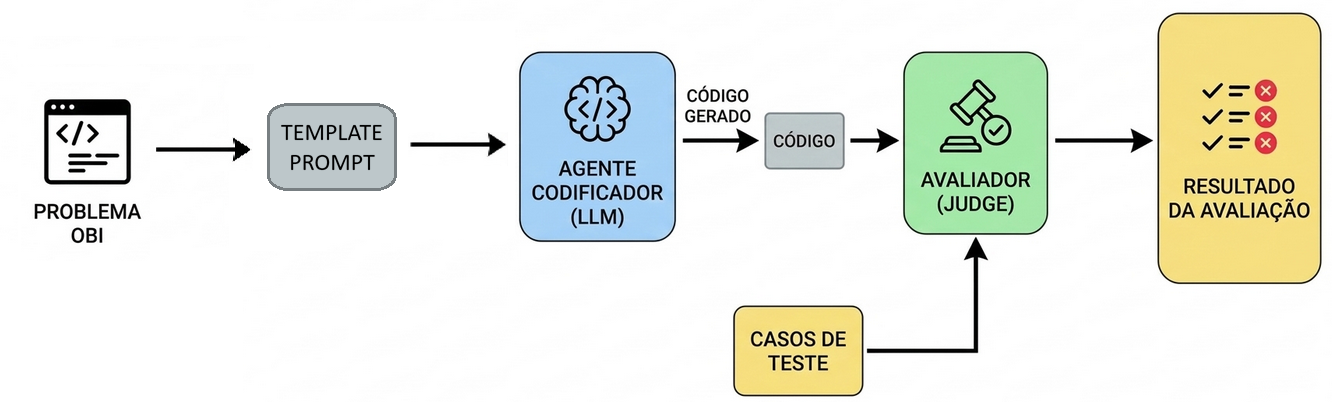
\includegraphics[width=0.8\textwidth]{figures/1.png}
\caption{Pipeline do sistema}
\label{fig:pipeline}
\end{figure}

\subsection{Banco de Problemas}

Para a realização dos experimentos, foi construído um banco de problemas (dataset) a partir do site oficial da Olimpíada Brasileira de Informática (OBI). A compilação e estruturação desse banco foram automatizadas por meio de um pipeline desenvolvido em Python, composto pelas seguintes cinco etapas:

\begin{itemize}
    \item \textbf{Coleta de Dados (Web Scraping):} Download dos cadernos de provas (abrangendo todos os níveis, de 2000 a 2025) utilizando a biblioteca \textit{requests} para requisições do conteúdo da página e \textit{BeautifulSoup} para a extração dos links.
    \item \textbf{Processamento via LLM:} Submissão dos arquivos PDF ao modelo Gemini 3.1 Pro para extração e estruturação dos dados em formato JSON. Os campos gerados incluíram: título, enunciado, entrada, saída, restrições, exemplos, pontuação, ano, nível, período e dificuldade (sendo este último atributo inferido pelo próprio modelo).
    \item \textbf{Obtenção dos Casos de Teste:} Download dos gabaritos oficiais (arquivos .zip) correspondentes a cada questão para extração das entradas e saídas esperadas.
    \item \textbf{Mapeamento de Arquivos:} Organização e vinculação dos casos de teste extraídos aos seus respectivos problemas no diretório do juiz automático (judge).
    \item \textbf{Limpeza e Validação:} Remoção de arquivos residuais e exclusão sumária das questões que não possuíam pareamento exato com os arquivos de entrada e saída, garantindo a integridade para a avaliação no judge.
\end{itemize}

Após a consolidação da base de dados, realizou-se uma análise exploratória do dataset, classificando os problemas sob dois critérios principais: (i) nível de dificuldade (fácil, médio e difícil); e (ii) domínio algorítmico, abrangendo tópicos como grafos, programação dinâmica, algoritmos gulosos e processamento de strings, entre outros \cite{obi2026}.

Ao final do processo foi feita uma análise manual para garantir que as questões de programação estavam com os gabaritos corretos e adicionando as imagens das respectivas questões, assim o banco de problemas tem uma amostragem validada no total de 493 questões no formato JSON \cite{anonimo2026}.

\subsection{Modelos Avaliados}

Os experimentos foram conduzidos utilizando diferentes modelos de linguagem multimodais, tal qual, são capazes de gerar código de programação a partir de descrições textuais e imagens. A seleção dos modelos utilizados (Claude Sonnet 4.6, Gemini 3.1 Pro, GPT 5.4, Mistral Small 4, Grok 4.20) tem como objetivo a avaliação do impacto nas imagens utilizadas no enunciado do problema na aplicação do problema de programação. Entretanto, houve uma segunda seleção dos modelos (Claude Sonnet 4.6, Gemini 3.1 Pro, GPT 5.4, DeepSeek-V3.2, Glm 5, Step 3.5 Flash, Grok Code Fast 1 e Mistral Small 4) com o objetivo de verificar os tipos de abordagens dos grandes modelos de linguagem que refletem não apenas o desempenho de imagens, mas no panorama geral atual da inteligência artificial generativa aplicada à programação competitiva.

\subsection{Ambiente de Avaliação}

Foi desenvolvido um ambiente experimental automatizado responsável por gerenciar todo o processo de avaliação das soluções geradas \cite{obibenchmarking2026} pelos modelos. O ambiente realiza as seguintes etapas na execução: escolha do ambiente de saída; execução de algum ano especifíco para questões da OBI; seleção de um problema do banco de dados no formato JSON; envio do enunciado ao modelo de linguagem; recebimento do código gerado pelo modelo; compilação e execução do código; avaliação automática utilizando casos de teste.

A verificação das soluções é realizada por meio da comparação entre a saída produzida pelo programa do modelo de IA e a saída esperada definida nos casos de teste do problema (Judge). Cada solução é classificada de acordo com categorias comuns em sistemas de juízes automáticos, como:

\begin{itemize}
    \item \textbf{Accepted (AC):} solução correta;
    \item \textbf{Wrong Answer (WA):} saída incorreta;
    \item \textbf{Compilation Error (CE):} erro de compilação;
    \item \textbf{Runtime Error (RE):} erro durante execução;
    \item \textbf{Time Limit Exceeded (TLE):} excedeu o limite de tempo.
\end{itemize}

Como os cadernos de problemas não especificam o tempo limite de execução nos testes, os casos de teste foram padronizados para 1 segundo para linguagem C++ e para 3 segundos para linguagem Python. Essa diferença existe devido aos paradigmas que ambas estão inseridas no contexto computacional. Enquanto a linguagem C++ tem seu tempo de execução otimizado devido a utilização de um compilador, o Python é executado linha por linha. Assim, no cenário da programação competitiva as linguagens interpretadas possuem um tempo maior que as linguagens que utilizam compiladores.

\section{Experimentos}

A condução dos experimentos engloba a orquestração das chamadas de API para LLMs com temperatura igual a 0, além do top\_p no valor padrão e o max\_tokens padrão para não restringir o tamanho do arquivo. Além disso, a submissão ao juiz automático (judge) e a medição do tempo de execução das soluções para o judge. Assim, o ambiente de hardware desses experimentos é constituído por um processador Intel Core i7-1360P de 13ª geração (2.20 GHz), 16 GB de memória RAM (4800 MT/s) e acelerador gráfico integrado Intel Iris Xe, operando sob o sistema Windows 11 Home (64 bits).

Com isso, a Seção 4.1 e a Seção 4.2 apresentam um experimento preliminar conduzido para determinar as configurações ótimas de geração. Nesta etapa, avaliou-se o desempenho dos modelos multimodais em relação a utilização de imagens, além do desempenho das linguagens Python e C++, bem como a eficácia das estratégias de prompting (zero-shot versus few-shot), uma vez que a escolha desses parâmetros afeta de maneira direta e significativa os resultados de acurácia e eficiência dos modelos avaliados neste estudo.

\subsection{Verificação de Imagens nos Enunciados}

Antes de iniciar a preparação do ambiente, foi necessário uma verificação dos modelos multimodais para entender o impacto que as imagens possuem para os modelos. Devido a isso, o enunciado possui referências às imagens como está exemplificado na figura \ref{fig:representacao}, durante a construção do prompt as imagens são transformadas para o formato Base64. Assim, os modelos multimodais conseguem extrair o conhecimento através da imagem, podendo impactar na geração do código e consequentemente o nível de acerto.

\begin{figure}[H]
\centering
\includegraphics[width=0.8\textwidth]{figures/2.png}
\caption{Representação do enunciado para os modelos de LLMs}
\label{fig:representacao}
\end{figure}

Com isso, o banco de problemas possui 181 questões com imagens, sendo 67 de nível fácil, 81 de nível médio e 33 de nível difícil. Ao analisar os códigos gerados pelos modelos com o número de acertos segundo o judge, é visível que não houve um ganho significativo nos ACs.

\begin{figure}[H]
\centering
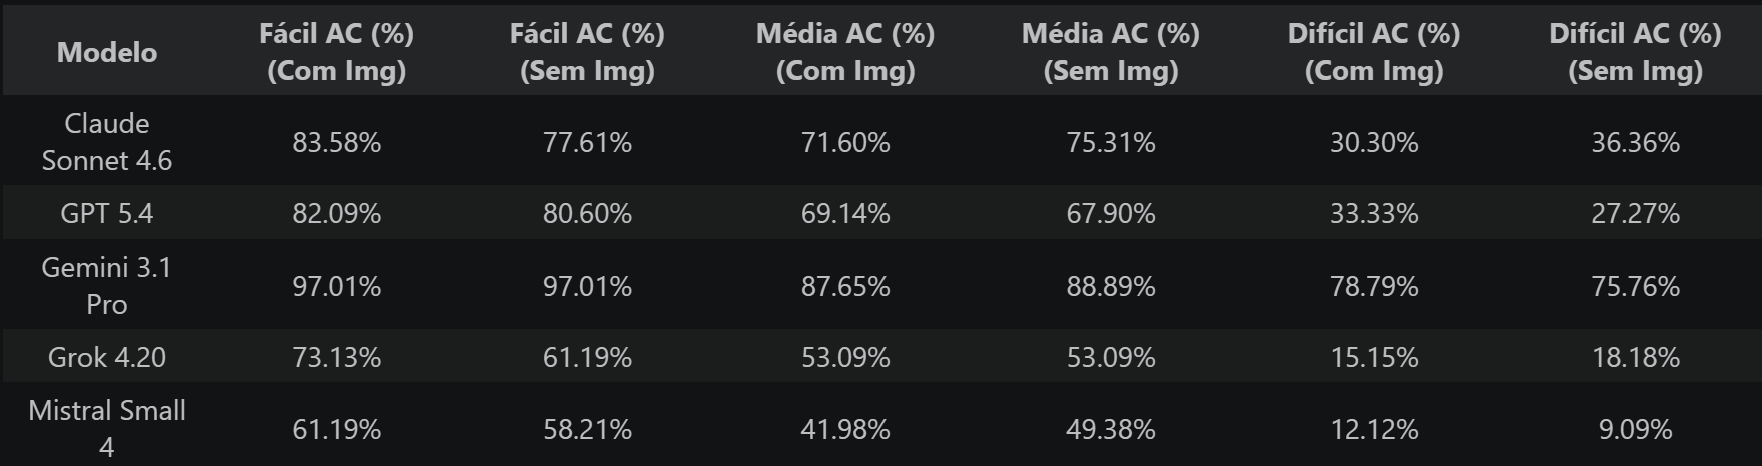
\includegraphics[width=0.8\textwidth]{figures/3.png}
\caption{Estatísticas enunciados com e sem imagens}
\label{fig:tabela1}
\end{figure}

Além disso, houve um aumento considerável na complexidade no tempo de geração de código pelos grandes modelos de linguagens. Além de aumentar o consumo dos tokens e consequentemente o custo médio dos prompts. Por isso, a configuração final utiliza apenas textos, pois como mostra a tabela 1 não é garantido que as imagens tenham impacto significativo nos modelos na produção de códigos.

\subsection{Preparação do Ambiente do Experimento}

Utilizando apenas os enunciados, o experimento busca verificar técnicas simples de prompt como o zero-shot e few-shot para melhor entendimento da performance dos modelos para técnicas básicas de prompt, tentando resolver 299 questões do banco de problemas, sendo 126 de nível fácil, 118 de nível médio e 55 de nível difícil. Devido a isso, em Kaplan et al. (2020) \cite{kaplan2020scaling}, foram estabelecidas leis de escala para modelos de linguagem, demonstrando que o aumento de parâmetros e de poder computacional impacta positivamente o desempenho geral. A partir dessa escalabilidade, as capacidades de aprendizado por exemplos (few-shot) tornaram-se viáveis nos LLMs. Contudo, Touvron et al. (2023) \cite{touvron2023llama} trouxeram uma nova perspectiva com o desenvolvimento do LLaMA, evidenciando que a excelência em tarefas de raciocínio (tanto em few-shot quanto em zero-shot) não depende exclusivamente de uma escala massiva de parâmetros, mas de um treinamento otimizado com um volume substancialmente maior de dados.

No experimento preliminar deste estudo, essas dinâmicas foram observadas na prática. Constatou-se que a abordagem zero-shot apresentou falhas frequentes na formatação estrita de entrada e saída exigida pelo juiz automático nas questões da OBI 2015. Para mitigar esse problema, adotou-se a técnica de few-shot fornecendo três exemplos de problemas (envolvendo grafos, soma simples e contagem em matriz) para guiar o agente codificador. Esse comportamento é coerente com a literatura revisada \cite{brown2020language}: os modelos utilizados neste benchmark possuem capacidade arquitetural suficiente para inferir padrões a partir dos exemplos no prompt, melhorando significativamente a compreensão do formato de I/O (entrada/saída) antes da geração da solução, conforme ilustrado na Figura \ref{fig:fewshot}.

\begin{figure}[H]
\centering
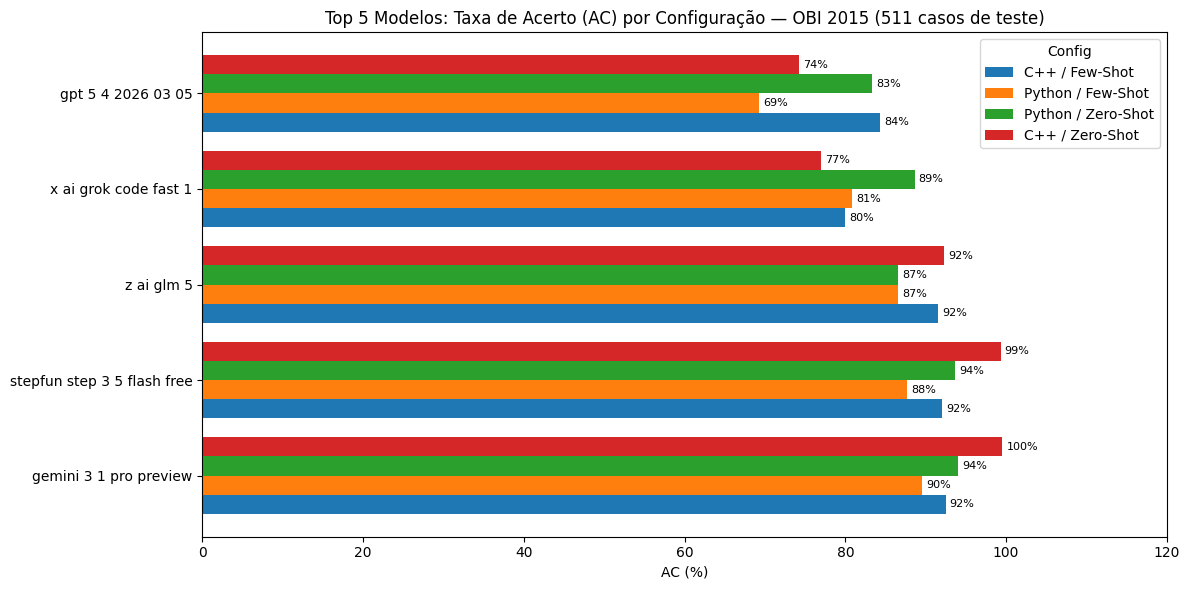
\includegraphics[width=0.8\textwidth]{figures/4.png}
\caption{Top 5 taxa de acertos dos casos de testes no judge em relação à linguagem de programação e a técnica de engenharia de prompt}
\label{fig:top5}
\end{figure}

Cabe ressaltar que este experimento preliminar avaliou 511 casos de teste. A configuração que obteve o melhor desempenho entre os cinco principais modelos avaliados foi a utilização da linguagem Python combinada à técnica "few-shot”. Consequentemente, esta foi a configuração metodológica adotada para a avaliação principal do presente artigo.

\subsection{Métricas de Avaliação}

Para a avaliação do desempenho dos modelos frente à base de dados composta pelas 299 questões da OBI, foram definidas métricas que mensuram tanto a eficácia na resolução algorítmica quanto a eficiência computacional e financeira. A análise comparativa fundamenta-se nos seguintes indicadores:

\begin{itemize}
    \item \textbf{Taxa de Sucesso (Acurácia):} Proporção de soluções que obtiveram aprovação integral em todos os casos de teste do juiz automático, estratificada pelos três níveis de dificuldade dos problemas.
    \item \textbf{Consumo de Tokens:} Média de tokens trafegados (somando o prompt de entrada e a solução gerada) por problema.
    \item \textbf{Custo de API:} Estimativa do gasto financeiro médio por requisição para a geração do código.
    \item \textbf{Latência de Inferência:} Tempo médio decorrido para a geração completa do código pelo modelo.
\end{itemize}

\section{Resultados e Discussões}

\subsection{Visão Geral do Desempenho}

Esta seção apresenta uma análise global dos resultados obtidos na submissão das 299 questões ao juiz automático. O objetivo deste levantamento inicial é fornecer um panorama das reais capacidades e limitações das ferramentas avaliadas, ponderando não apenas a taxa de acerto absoluto, mas também a viabilidade prática em termos de latência e custo financeiro.

A avaliação das 299 questões revelou que parte dos modelos falhou na geração de códigos sintaticamente válidos, um fenômeno observado predominantemente nos problemas de nível difícil. Esse resultado evidencia que a alta complexidade algorítmica inerente à programação competitiva ainda representa uma barreira substancial para a capacidade de síntese de código executável por essas ferramentas.

\begin{figure}[H]
\centering
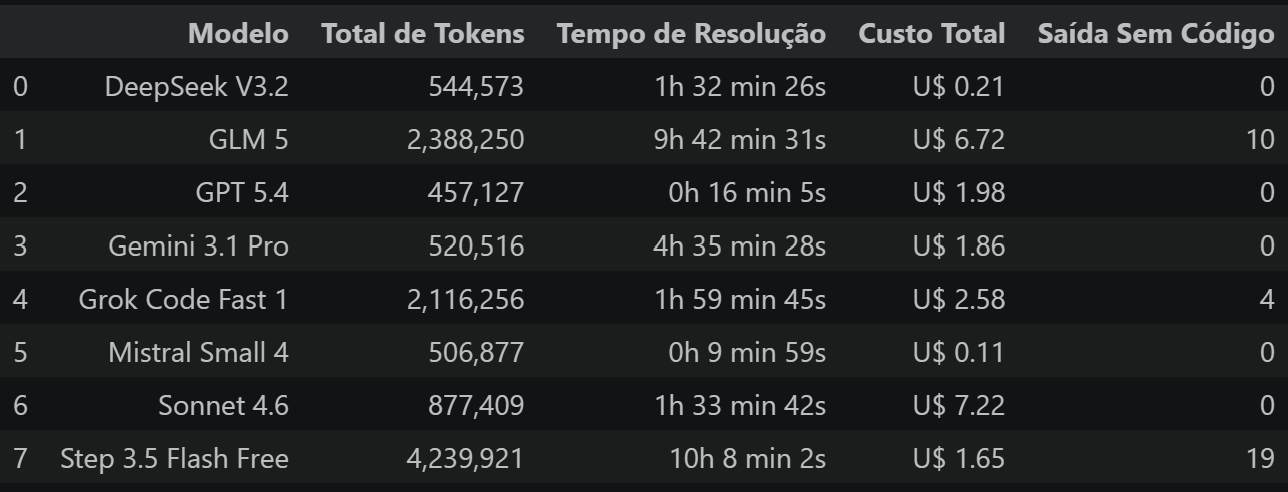
\includegraphics[width=0.8\textwidth]{figures/5.png}
\caption{Estatísticas da execução do experimento}
\label{fig:tabela2}
\end{figure}

Adicionalmente, a análise indicou uma ausência de correlação direta entre o custo de inferência e o desempenho algorítmico no juiz automático (judge). Modelos de maior custo financeiro não apresentaram, necessariamente, as maiores taxas de sucesso. Nesse contexto, conforme os dados da Tabela 2, os modelos GPT 5.4 e Grok Code Fast 1 destacaram-se por sua baixa latência, configurando-se como opções adequadas e ágeis para a resolução de problemas de níveis fácil e médio.

\begin{figure}[H]
\centering
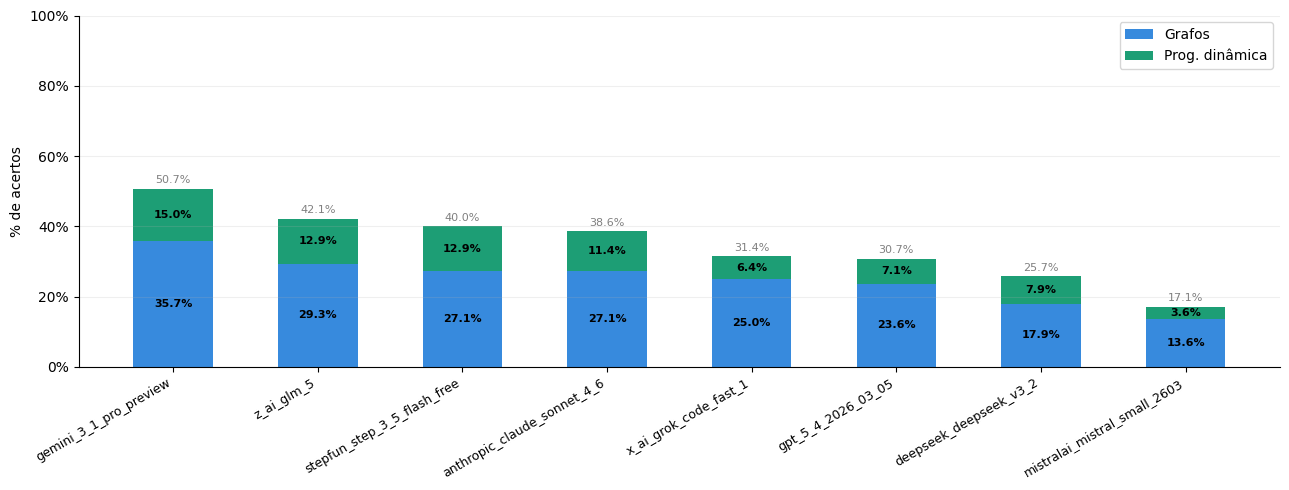
\includegraphics[width=0.8\textwidth]{figures/6.png}
\caption{Taxa de acerto nos tópicos programação dinâmica e grafos}
\label{fig:topicos}
\end{figure}

Veja que para os problemas de grafos e programação dinâmica não houve um bom desempenho dos modelos. Tal que, apenas o modelo Gemini 3.1 Pro teve uma taxa de acerto 82,70\%, logo esse é o modelo recomendado para problemas com esses tópicos.

\begin{figure}[H]
\centering
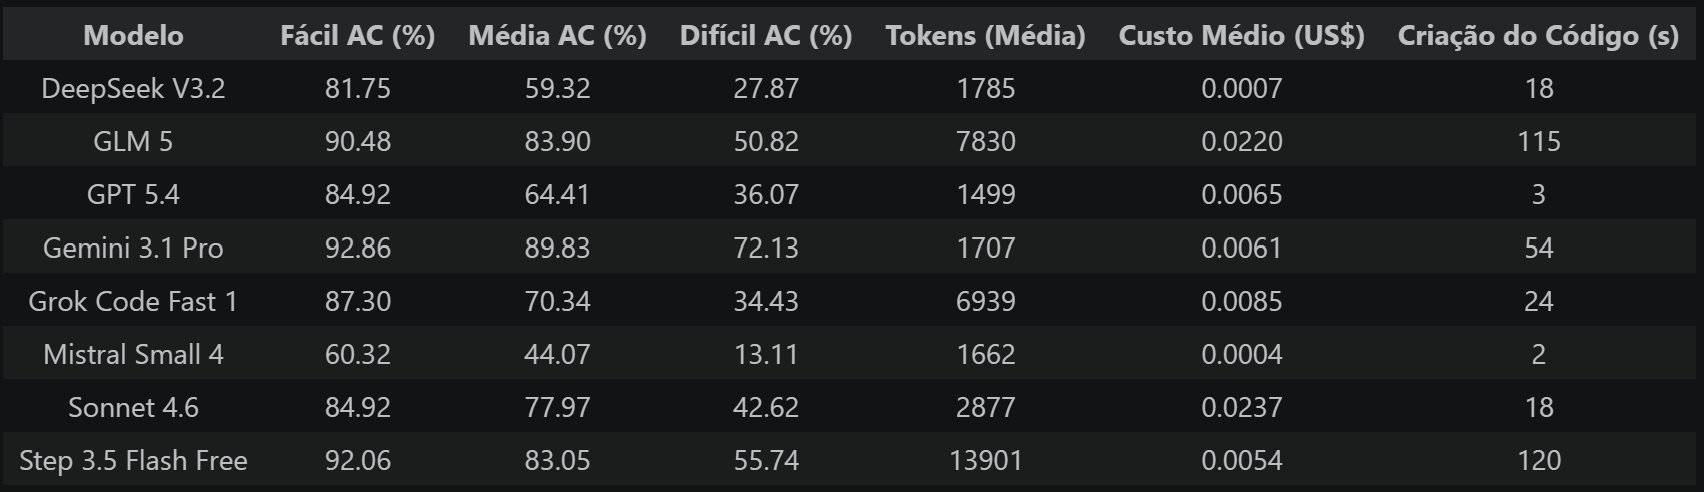
\includegraphics[width=0.8\textwidth]{figures/7.png}
\caption{Benchmarking modelos de LLMs resolvendo questões}
\label{fig:tabela3}
\end{figure}

Por fim, o modelo Gemini 3.1 Pro demonstrou a melhor relação custo-benefício do experimento. A ferramenta atingiu as maiores taxas de acerto globais no judge, mantendo um custo médio competitivo em comparação a modelos como Claude Sonnet 4.6 e GLM 5. Sua única limitação expressiva foi a latência, registrando o terceiro maior tempo médio de geração por problema. Em contrapartida, o modelo Mistral Small 4 apresentou o desempenho mais baixo do estudo. Em um espectro oposto, o modelo Step 3.5 Flash Free destacou-se positivamente ao alcançar taxas de sucesso comparáveis ou superiores às de modelos comerciais pagos, apesar de operar com uma arquitetura reduzida de 11 bilhões de parâmetros ativos.

\subsection{Taxa de Acerto nos Níveis de Dificuldade}

Os agentes codificadores tiveram um desempenho considerado alto para questões fáceis (acima de 85\%, menos Mistral Small 4) e médias (acima de 62\%, menos Mistral Small 4), tal que, são questões menos complexas que não precisam de pré-processamento das entradas ou apenas 1 técnica de programação para conseguir chegar na saída esperada.

Porém, como as LLMs ainda têm certa dificuldade para ter uma cobertura total nas questões difíceis, mostra que buscar conhecimento nas LLMs não é garantido que o mesmo consiga responder a questão, principalmente para questões de programação competitiva. Assim, intervenções estruturas para lidar com conceitos complexos, exigindo abordagens pedagógicas direcionadas para cada perfil de estudante \cite{baist2017analysis}, fazem-se estritamente necessárias ao integrar a Inteligência Artificial no ensino.

Portanto, esse cenário é evidenciado pelos dados de desempenho do próprio modelo Claude Sonnet 4.6, que, embora atinja taxas de sucesso de 83,05\% e 88,89\% em problemas de nível fácil e médio, sofre uma queda abrupta para apenas 45,90\% em questões difíceis. Isso demonstra que a Inteligência Artificial está evoluindo ao transitar da sintaxe básica para o raciocínio algorítmico complexo, mas é preciso cautela.

\section{Conclusão}

Este artigo apresentou uma avaliação experimental abrangente da capacidade de diferentes Modelos de Linguagem de Grande Escala (LLMs) na resolução de problemas de programação, utilizando como benchmark a Olimpíada Brasileira de Informática (OBI). O ambiente automatizado desenvolvido permitiu quantificar não apenas a correção sintática do código gerado, mas também a eficácia lógica e algorítmica frente a casos de teste rigorosos.

Os resultados demonstram que modelos como GLM 5, Sonnet 4.6, Step 3.5 Flash Free, GPT 5.4, DeepSeek V3.2 apresentam domínio em problemas de nível básico e intermediário, mas existe uma degradação acentuada da performance em questões que exigem raciocínio algorítmico complexo, especificamente em problemas envolvendo grafos e programação dinâmica. Isso é visível através do gargalo autorregressivo que as LLMs possuem, pois ao produzir uma saída palavra por palavra, da esquerda para a direita, a mesma não consegue reavaliar o que já escreveu no mesmo output. Além disso, essa linearidade de geração do código acaba impactando diretamente em pontos como tempo de execução, gerenciamento da memória, erros de compilação dos códigos.

A investigação também revelou que a abordagem multi-agente, observada no modelo Grok Code Fast 1, superou as configurações de agente único em cenários de exploração inicial, ou seja, para problemas de programação competitiva como na modalidade programação da OBI os modelos de único agente cometem erros na codificação, pois os enunciados são grandes, possui um raciocínio lógico complexos e precisa que a sintaxe da linguagem esteja correta, no qual podem ser separados em sub-agentes especializados como o Grok Code Fast 1 busca essa otimização, tendo uma taxa de sucesso de 92,06\% em questões de nível de dificuldade fácil. Por outro lado, o Gemini 3.1 Pro Preview destacou-se pela consistência técnica, especialmente com a linguagem Python. Evidenciou-se também que o uso de few-shot prompting é uma estratégia essencial de alinhamento para mitigar erros de formatação de entrada e saída, embora o aumento no contexto possa introduzir latência adicional no pipeline de geração.

Em última análise, este estudo reafirma que, apesar do potencial dos LLMs como ferramentas de apoio, a especialização humana em programação competitiva permanece indispensável. Os modelos atuais funcionam melhor como assistentes de produtividade do que como resolvedores autônomos de problemas complexos.

Como desdobramento desta pesquisa, propõe-se ampliar a avaliação experimental para um banco de questões de olimpíadas com mais variedade de problemas e estilos diferentes como a modalidade iniciação.

\bibliographystyle{sbc}
\bibliography{sbc-template}

\section{Anexos}

A seguir mostra-se um detalhamento sobre prompts utilizado, incluindo templates.

\subsection{Zero-shot prompt}

\begin{figure}[H]
\centering
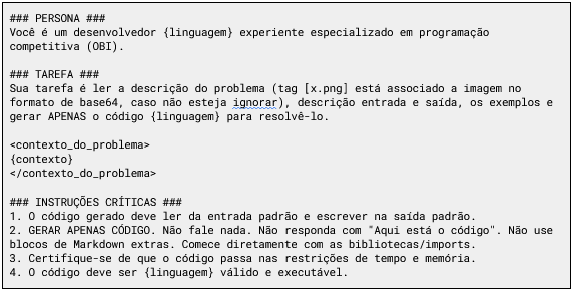
\includegraphics[width=0.8\textwidth]{figures/8.png}
\caption{Prompt Zero-shot para o Agente Codificador}
\end{figure}

\subsection{Few-shot prompt}

\begin{figure}[H]
\centering
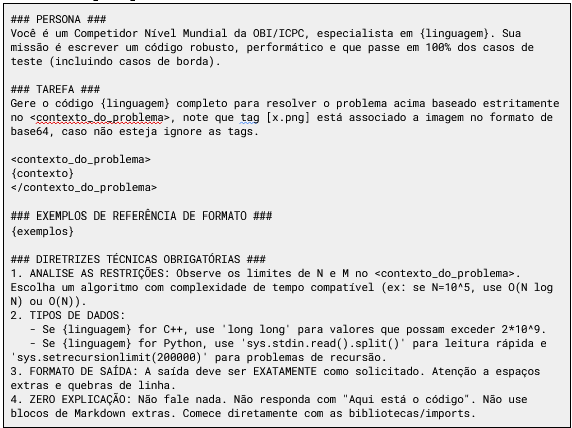
\includegraphics[width=0.8\textwidth]{figures/9.png}
\caption{Prompt Few-shot para o Agente Codificador}
\label{fig:fewshot}
\end{figure}

\end{document}
